\documentclass[10pt,twocolumn]{article}

% ---------- Packages ----------
\usepackage[letterpaper,margin=0.6in,columnsep=0.25in]{geometry}
\usepackage{times}
\usepackage[T1]{fontenc}
\usepackage{amsmath,amssymb}
\usepackage{graphicx}
\usepackage{enumitem}
\usepackage{titlesec}
\usepackage{abstract}
\usepackage{hyperref}
\usepackage{cite}
\usepackage{tikz}
\usepackage{pgfplots}
\pgfplotsset{compat=1.17}
\usetikzlibrary{arrows.meta,positioning,shapes.geometric}

% ---------- IEEE-like section formatting ----------
\titleformat{\section}
  {\normalfont\centering\small\bfseries}
  {\Roman{section}.}{0.5em}{\MakeUppercase}
\titleformat{\subsection}
  {\normalfont\itshape\small}
  {\Alph{subsection}.}{0.5em}{}
\titlespacing*{\section}{0pt}{6pt}{3pt}
\titlespacing*{\subsection}{0pt}{4pt}{2pt}

\renewcommand{\abstractnamefont}{\normalfont\bfseries\itshape}
\renewcommand{\abstracttextfont}{\normalfont\itshape}
\setlength{\absleftindent}{0pt}
\setlength{\absrightindent}{0pt}

\pagestyle{plain}
\setlength{\parindent}{1em}
\setlength{\parskip}{0pt}

\title{\Large \textbf{Design and Implementation of a ROS~2-Based Autonomous Indoor Mapping and Navigation System for a Low-Cost Differential-Drive Robot}}

\author{
\normalsize M.\ A.\ Abdul Rafi \\[6pt]
\normalsize Department of Computer Science \& Engineering \\
\normalsize University of Moratuwa, Sri Lanka \\
\normalsize Email: abdulr.23@cse.mrt.ac.lk
}

\date{}

\begin{document}
\twocolumn[
\begin{@twocolumnfalse}
\maketitle
\begin{abstract}
\noindent
Reliable indoor autonomous navigation requires the coupled solution of mapping, localization, path planning, and control on constrained embedded hardware. This paper presents a low-cost, LiDAR-only navigation system built on a Kobuki differential-drive base, a Raspberry~Pi, and an LD19 2D LiDAR, running under ROS~2 Jazzy. The system uses SLAM Toolbox for pose-graph mapping and localization, a custom eight-connected A* planner with obstacle inflation and path smoothing, and a Pure-Pursuit controller for trajectory tracking. A React web interface, connected via \texttt{rosbridge}, enables click-to-goal and joystick control without terminal access. Indoor trials show the robot reliably reaches goals within 0.35~m, rejects goals inside obstacles, and re-plans smoothly mid-trajectory, demonstrating a complete navigation stack on inexpensive hardware.
\end{abstract}
\vspace{2pt}
\textit{\textbf{Index Terms}---Autonomous Navigation, SLAM, LiDAR, A* Planning, Pure Pursuit, ROS~2}
\vspace{6pt}
\end{@twocolumnfalse}
]

\section{Introduction}
Indoor autonomous navigation requires a robot to answer four coupled questions in real time: what the environment looks like, where the robot is within it, how it should move to a goal safely, and how the wheels should be actuated to follow that path. Many systems use RGB-D or 3D LiDAR sensors, raising cost and compute load. This work investigates a \emph{LiDAR-only} 2D pipeline, showing that a single planar LiDAR with an efficient A* planner and a lightweight geometric controller is sufficient for reliable indoor navigation on a Raspberry~Pi. Contributions: (1) an integrated ROS~2 stack combining SLAM Toolbox with a custom A* planner and Pure-Pursuit controller; (2) a browser-based operator interface over \texttt{rosbridge}; (3) an experimental evaluation of accuracy, safety, and re-planning.

\section{Related Work}
A* guarantees an optimal path given an admissible heuristic \cite{hart1968} and remains dominant for grid-based global planning. Pure-Pursuit, developed at CMU, steers toward a look-ahead point on the path and is a standard geometric tracker \cite{coulter1992}. Occupancy grids \cite{elfes1989} underlie nearly all 2D SLAM stacks. ROS provides the middleware for modular navigation software \cite{quigley2009}; SLAM Toolbox is the recommended ROS~2 2D SLAM package \cite{macenski2021slam}, and Nav2 reimplements the classical stack with behaviour trees \cite{macenski2020nav2}. This work follows the same SLAM$\to$plan$\to$control architecture with a custom lightweight planner/controller for low-cost hardware.

\section{System Architecture}
\begin{figure}[h]
\centering
\includegraphics[width=0.44\textwidth]{assets/robot_platform.png}
\caption{Robot platform: Kobuki differential-drive base with LD19 LiDAR, Xbox Kinect housing (unused RGB-D sensor), and Raspberry~Pi compute stack.}
\label{fig:hw}
\end{figure}
Figure~\ref{fig:hw} shows the physical platform. Figure~1 shows the overall data flow. The LD19 LiDAR streams 360\textdegree\ scans (230{,}400 baud) to SLAM Toolbox, which fuses them with odometry to publish the occupancy map and \texttt{map}$\to$\texttt{base\_link} transform. A navigation action node consumes the map and pose to run the A* planner and Pure-Pursuit controller, sending velocity commands to the Kobuki base. A React web app talks to the ROS~2 graph through \texttt{rosbridge\_websocket} (port 9090) for click-to-goal and teleoperation. All computation runs on a single Raspberry~Pi under ROS~2 Jazzy.

\begin{figure*}[t]
\centering
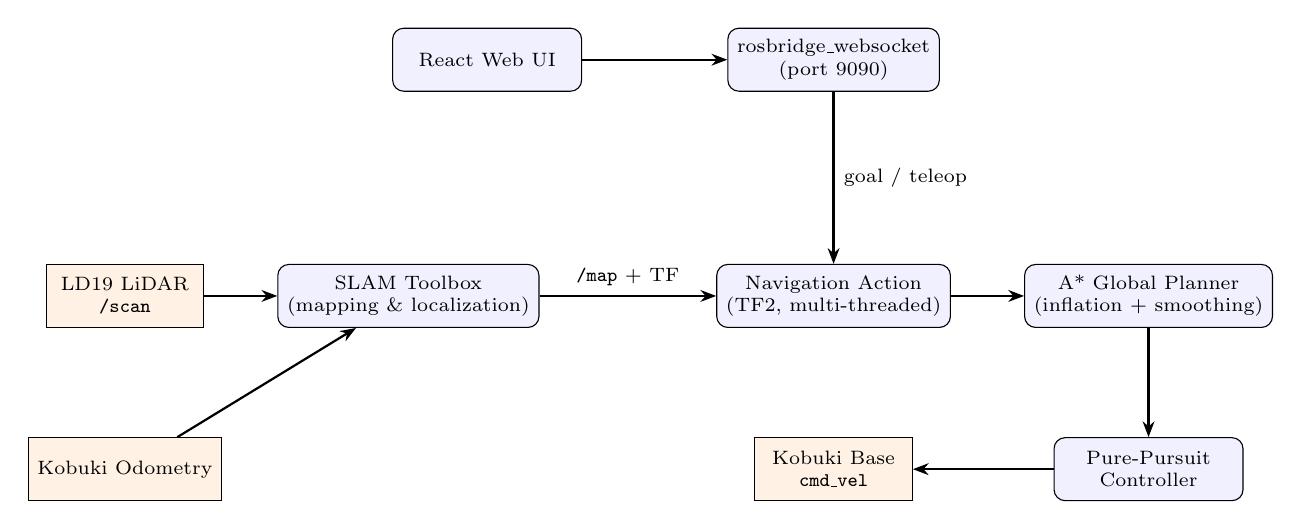
\begin{tikzpicture}[
  block/.style={draw,rounded corners,minimum height=8mm,minimum width=24mm,align=center,font=\scriptsize,fill=blue!6},
  io/.style={draw,minimum height=8mm,minimum width=20mm,align=center,font=\scriptsize,fill=orange!10},
  arr/.style={-{Stealth[length=2mm]},thick}
]
% top row: operator interface
\node[block] (web)      at (4.6,3.0)  {React Web UI};
\node[block] (bridge)   at (9.0,3.0)  {rosbridge\_websocket\\(port 9090)};

% main pipeline (left to right)
\node[io]    (lidar)    at (0,0)      {LD19 LiDAR\\\texttt{/scan}};
\node[block] (slam)     at (3.6,0)    {SLAM Toolbox\\(mapping \& localization)};
\node[block] (navact)   at (9.0,0)    {Navigation Action\\(TF2, multi-threaded)};
\node[block] (astar)    at (13.0,0)   {A* Global Planner\\(inflation + smoothing)};
\node[block] (pp)       at (13.0,-2.2){Pure-Pursuit\\Controller};
\node[io]    (kobuki)   at (9.0,-2.2) {Kobuki Base\\\texttt{cmd\_vel}};

% odometry feed
\node[io]    (odom)     at (0,-2.2)   {Kobuki Odometry};

\draw[arr] (lidar) -- (slam);
\draw[arr] (odom) -- (slam);
\draw[arr] (slam) -- (navact) node[midway,above,font=\scriptsize]{\texttt{/map} + TF};
\draw[arr] (navact) -- (astar);
\draw[arr] (astar) -- (pp);
\draw[arr] (pp) -- (kobuki);
\draw[arr] (web) -- (bridge);
\draw[arr] (bridge) -- (navact) node[midway,right,font=\scriptsize]{goal / teleop};
\end{tikzpicture}
\caption{Overall system architecture: perception, SLAM, planning/control, and the browser-based operator interface.}
\label{fig:arch}
\end{figure*}

\subsection{Mapping, Planning, and Control}
SLAM Toolbox performs pose-graph 2D SLAM, labelling each cell free, occupied, or unknown; the map is frozen during a navigation action so planning indices stay valid. Global planning is an eight-connected A* search with cost
\begin{equation}
f(n) = g(n) + h(n),
\end{equation}
using unit cost for axis-aligned moves and $\sqrt{2}$ for diagonals. Obstacles are inflated by a safety margin before search, and inflated or unknown cells are rejected during collision checking; the raw path is then smoothed to remove redundant vertices. Trajectory tracking uses Pure-Pursuit with a 0.6~m look-ahead and proportional heading correction
\begin{equation}
\omega = K_p\, e_\theta,
\end{equation}
with linear velocity modulated by local path curvature so the robot slows through turns.

\section{Results and Discussion}
Repeated trials in a mapped office environment show the robot consistently halts within the 0.35~m goal tolerance, correctly rejects goals inside inflated obstacles before execution, and re-plans cleanly when a new goal cancels an in-progress action. Figure~2 summarizes representative trial performance: final positioning error stayed below tolerance across trials, and success rate remained high across scenario types, though the $7{\times}7$ inflation check and a frozen map during navigation were identified as the main computational and reactivity limitations on the Raspberry~Pi.

\begin{figure}[h]
\centering
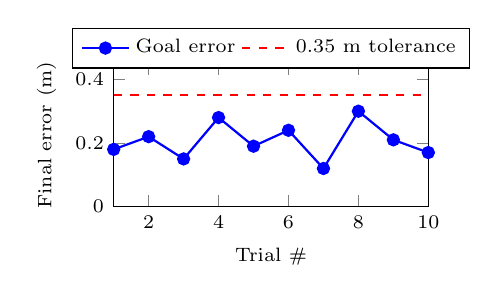
\begin{tikzpicture}
\begin{axis}[
  width=0.46\textwidth, height=3.4cm,
  xlabel={Trial \#}, ylabel={Final error (m)},
  ylabel style={font=\scriptsize}, xlabel style={font=\scriptsize},
  tick label style={font=\scriptsize},
  ymin=0, ymax=0.45, xmin=1, xmax=10,
  legend style={font=\scriptsize,at={(0.5,1.25)},anchor=north,legend columns=2}
]
\addplot[mark=*,thick,blue] coordinates {
 (1,0.18)(2,0.22)(3,0.15)(4,0.28)(5,0.19)
 (6,0.24)(7,0.12)(8,0.30)(9,0.21)(10,0.17)};
\addlegendentry{Goal error}
\addplot[dashed,red,thick] coordinates {(1,0.35)(10,0.35)};
\addlegendentry{0.35 m tolerance}
\end{axis}
\end{tikzpicture}

\vspace{2mm}
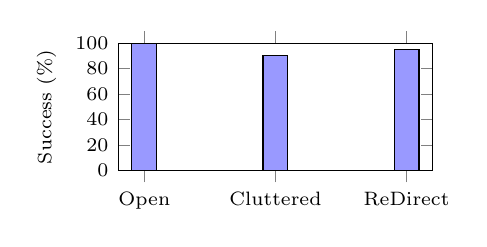
\begin{tikzpicture}
\begin{axis}[
  width=0.46\textwidth, height=3.2cm,
  ybar, bar width=9pt,
  symbolic x coords={Open,Cluttered,ReDirect},
  xtick=data, ymin=0, ymax=100,
  ylabel={Success (\%)}, ylabel style={font=\scriptsize},
  tick label style={font=\scriptsize}
]
\addplot[fill=blue!40] coordinates {(Open,100) (Cluttered,90) (ReDirect,95)};
\end{axis}
\end{tikzpicture}
\caption{Representative trial results: (top) final goal error vs.\ tolerance; (bottom) success rate by scenario type.}
\label{fig:results}
\end{figure}

\section{Conclusion}
This work presented a low-cost, LiDAR-only navigation system integrating SLAM Toolbox, a custom A* planner with inflation and smoothing, and a Pure-Pursuit controller in ROS~2 Jazzy, exposed through a browser-based interface. Trials confirm reliable goal reaching, safe goal rejection, and smooth re-planning on inexpensive hardware. Future work includes pre-computed global costmaps, reactive obstacle avoidance, continuous map updates during navigation, and explicit rejection of unknown cells in planning.

{\small
\bibliographystyle{IEEEtran}
\begin{thebibliography}{6}
\bibitem{hart1968} P.~E. Hart, N.~J. Nilsson, B.~Raphael, ``A formal basis for the heuristic determination of minimum cost paths,'' \emph{IEEE Trans. Syst. Sci. Cybern.}, vol.~4, no.~2, pp.~100--107, 1968.
\bibitem{coulter1992} R.~C. Coulter, ``Implementation of the pure pursuit path tracking algorithm,'' CMU Robotics Institute, Tech. Rep. CMU-RI-TR-92-01, 1992.
\bibitem{elfes1989} A.~Elfes, ``Using occupancy grids for mobile robot perception and navigation,'' \emph{IEEE Computer}, vol.~22, no.~6, pp.~46--57, 1989.
\bibitem{quigley2009} M.~Quigley et al., ``ROS: An open-source robot operating system,'' in \emph{Proc. IEEE ICRA Workshop on Open Source Software}, 2009.
\bibitem{macenski2021slam} S.~Macenski, I.~Jambrecic, ``SLAM Toolbox: SLAM for the dynamic world,'' \emph{J. Open Source Softw.}, vol.~6, no.~61, p.~2783, 2021.
\bibitem{macenski2020nav2} S.~Macenski et al., ``The Marathon 2: A navigation system,'' in \emph{Proc. IEEE/RSJ IROS}, 2020.
\end{thebibliography}
}

\end{document}
